\documentclass[12pt]{article}
\usepackage[hmargin=1.25in, vmargin=1.1in]{geometry}

\usepackage[utf8]{inputenc}
\usepackage[T1]{fontenc}
\usepackage[francais]{babel}
\usepackage{enumitem}% http://ctan.org/pkg/enumitem
\usepackage{listings}
\usepackage{color}
\usepackage{graphicx}
\usepackage{float}
\usepackage{upquote}
\usepackage{lastpage}
\usepackage{fancyhdr}
\pagestyle{fancy}
\usepackage{longtable}
\usepackage{tabu}
\usepackage{pdflscape}
\graphicspath{ {images/} }

\newcommand{\helv}{\fontfamily{phv}\fontseries{b}\fontsize{9}{11}\selectfont}



%--------------- Variables à modifier à chaque rendu ---------------
\title{Rendu 3}
\newcommand{\daterendu}{15/11/2017}
%-------------------------------------------------------------------
\setlist[itemize]{noitemsep, topsep=1pt}
\makeatletter\let\Title\@title\makeatother

% Décommenter pour commencer les chapitres à 0
%\setcounter{section}{-1}


%----------------------------------------------------------------------------------------
% CODE DISPLAY
%----------------------------------------------------------------------------------------

\lstset{
 language=Java,
 basicstyle=\ttfamily,
 keywordstyle=\color{purple},
 stringstyle=\color{red},
 commentstyle=\color{green},
 morecomment=[s][\color{blue}]{/**}{*/},
 tabsize=3,
 showspaces=false,
 %frame=single,
 showstringspaces=false,
 keywordstyle={[2]\color{red}\bf},
 inputencoding=utf8,
 breaklines=true,
 extendedchars=true,
 literate={à}{{\`a}}1 {ê}{{\^e}}1 {é}{{\'e}}1 {è}{{\'e}}1 {ô}{{\^o}}1 {î}{{\^i}}1 {ç}{{\c{c}}}1 {delta}{{\tiny$\Delta$}}1
}



\begin{document}

\begin{titlepage}

\newcommand{\HRule}{\rule{\linewidth}{0.5mm}} % Defines a new command for the horizontal lines, change thickness here

\center % Center everything on the page



\includegraphics[width=\textwidth]{logo_HEIA.jpg}\\[1.3cm]
\textsc{\Large Génie Logiciel 2 \\ [0.4cm]
\large Automne 2016-2017 \\ [0.4cm]
\large Mini-Projet SimuLife}\\[1.8cm] 


\textsc{
\bfseries \LARGE Water World\\ [0.8cm]
\Large Groupe No : 6}\\[1.4cm]


\HRule \\[0.4cm]
{ \huge \bfseries \Title }\\ 
\HRule \\[1.2cm]

\Large 
Bastien \textsc{Monney}\\[0cm]
Nicolas \textsc{Fuchs}\\[0cm]
Guillaume \textsc{Michel}\\[1.7cm] 

{\large Date du rendu : \daterendu}\\[1.5cm] 

\begin{center}
\large Enseignant : Pierre Kuonen / Julien Tscherrig
\end{center}

\end{titlepage}
\pagenumbering{Roman}

\renewcommand{\headrulewidth}{1pt}
\fancyhead[L]{\helv WaterWorld}
\fancyhead[C]{\helv 2017-2018}
\fancyhead[R]{\helv \Title }

\renewcommand{\footrulewidth}{1pt}
\fancyfoot[C]{\helv Table des matières \thepage{}}

\setcounter{page}{1}

\begin{center}
\renewcommand{\contentsname}{Table des matières}
\tableofcontents
\end{center}

\newpage
 {\setlength{\baselineskip}{1.5\baselineskip}
\fancyhf{}
\renewcommand{\headrulewidth}{1pt}
\fancyhead[L]{\helv Nom du Groupe}
\fancyhead[C]{\helv 2016-2017}
\fancyhead[R]{\helv \Title }

\renewcommand{\footrulewidth}{1pt}
\fancyfoot[L]{\helv GL2-Info, Automne 2017 - 2018}
\fancyfoot[C]{}
\fancyfoot[R]{\helv \textbf{Page \thepage{} sur \pageref{LastPage}}}
\pagenumbering{arabic}
\setcounter{page}{1}

\clearpage\pagestyle{empty}
\begin{landscape}
	\section{Diagramme de classe}
		On peut voir ici en vert le pattern observeur, en jaune le pattern Factory ainsi qu'en orange le pattern singleton. Le pattern command est mis en évidence à la fin de ce document.\newline
	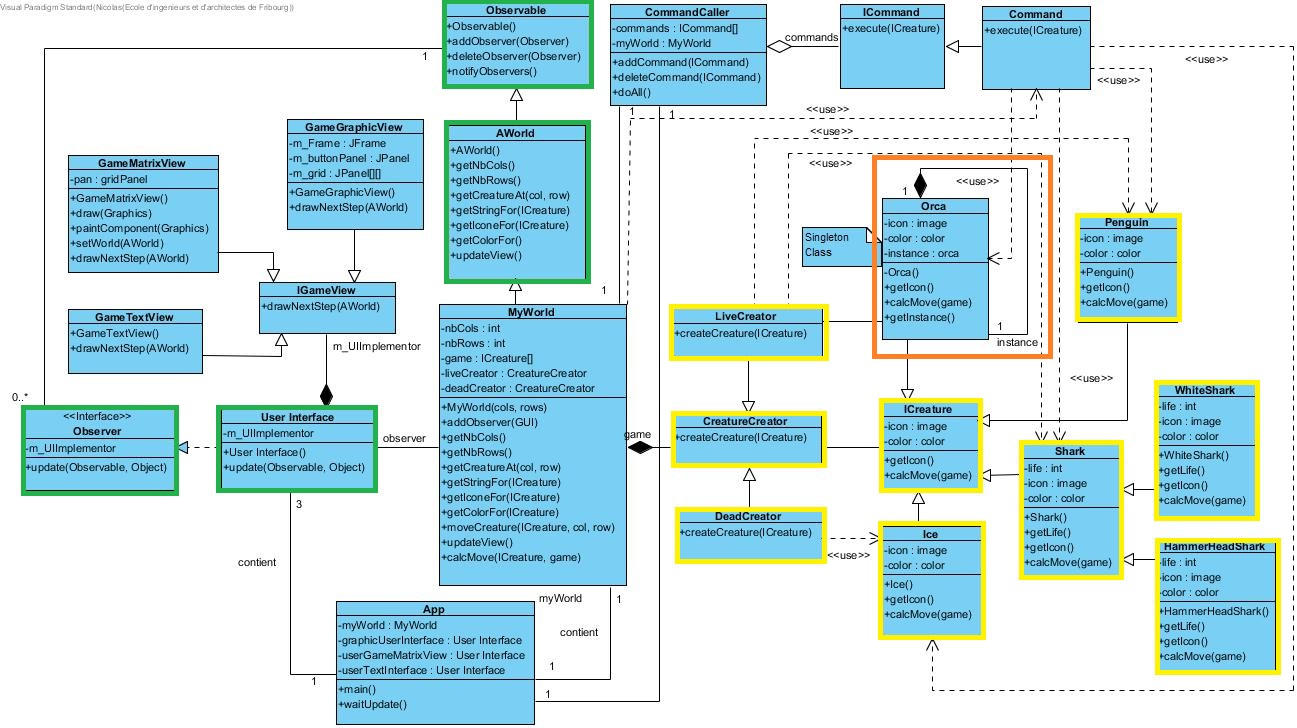
\includegraphics[scale=0.8]{Class.jpg}
\end{landscape}


\clearpage\pagestyle{empty}
\begin{landscape}
	\section{Diagramme de séquence}
	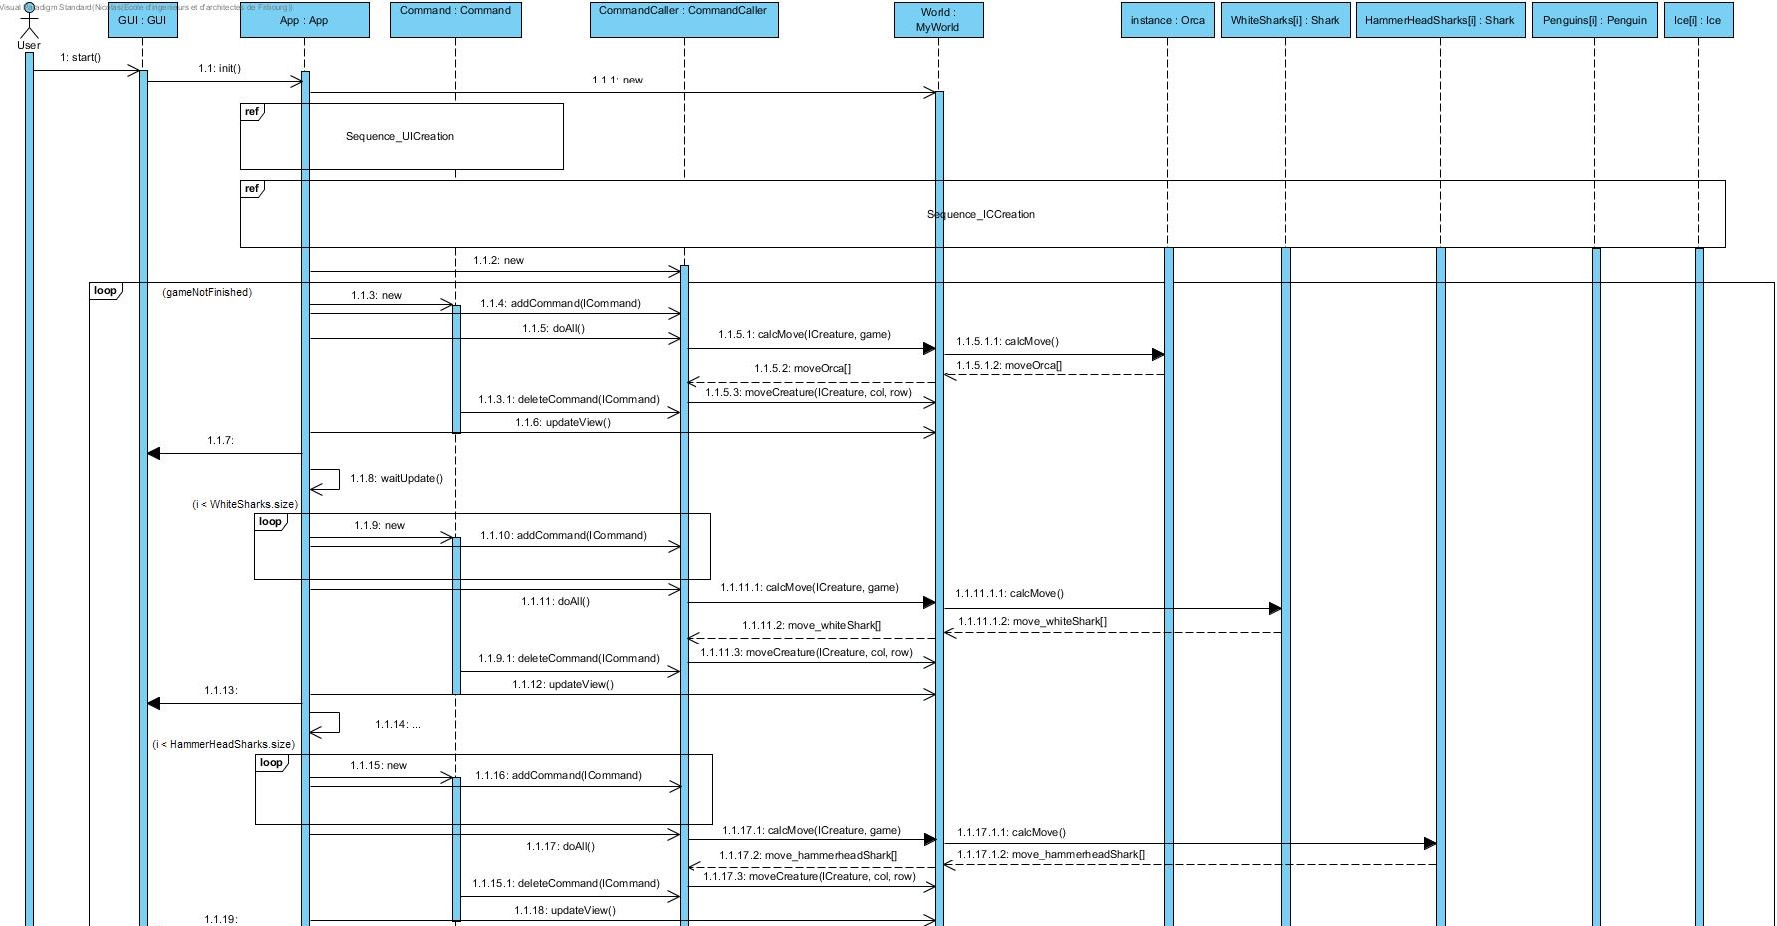
\includegraphics[scale=0.52]{Sequence.jpg}
\end{landscape}
	
\clearpage\pagestyle{empty}
\begin{landscape}
	\section{Diagramme de séquence}
	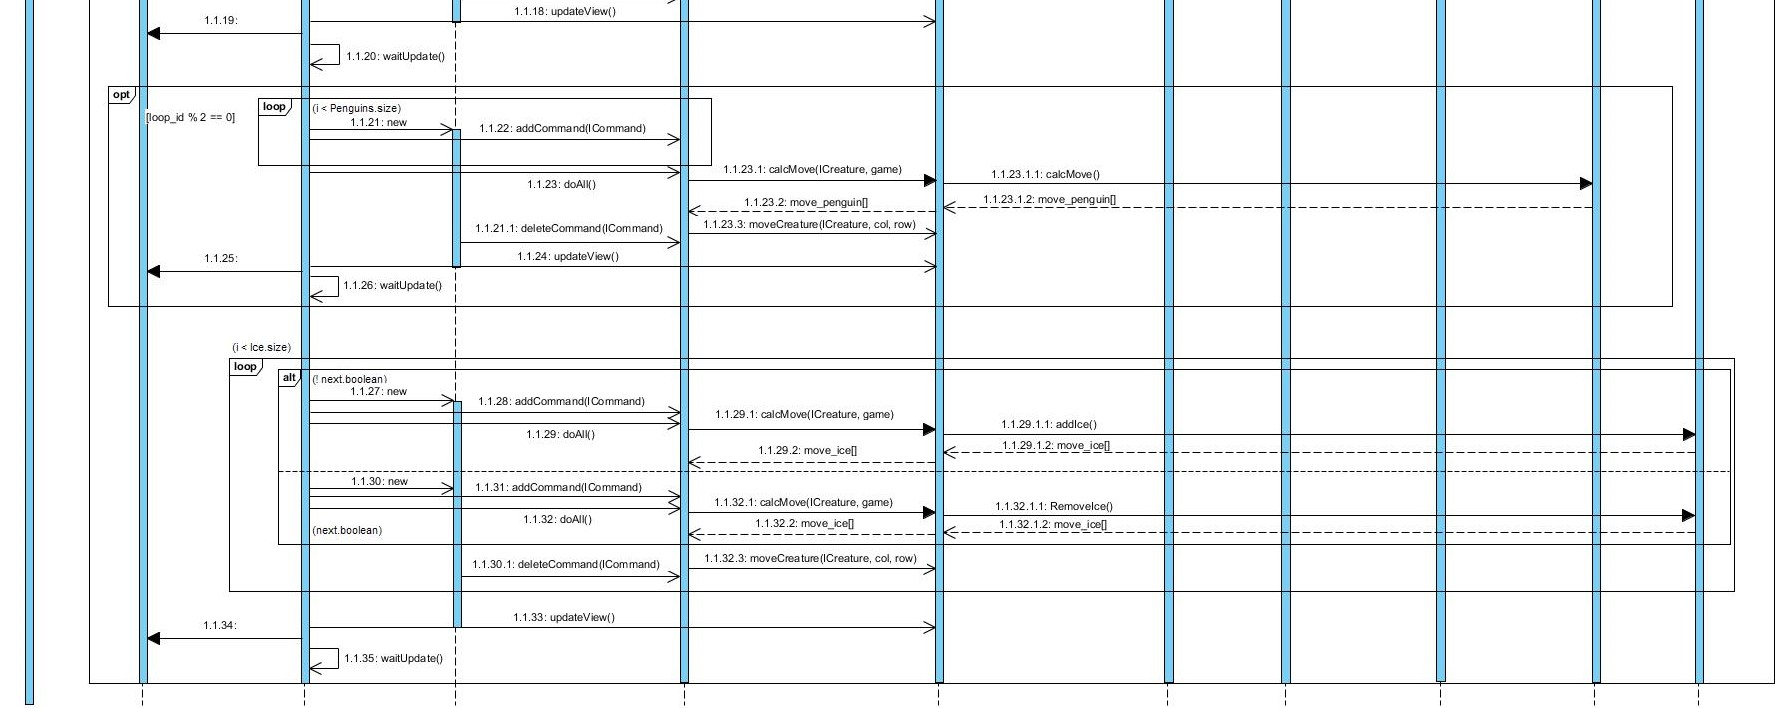
\includegraphics[scale=0.52]{Sequence2.jpg}
\end{landscape}


\clearpage\pagestyle{empty}
\begin{landscape}
	\section{Diagramme de séquence}
	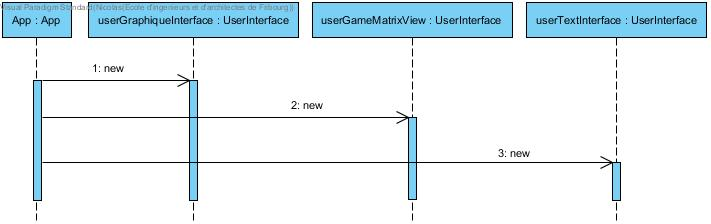
\includegraphics[scale=0.4]{Sequence_r1.jpg}\newline
\rule{\linewidth}{.5pt}
	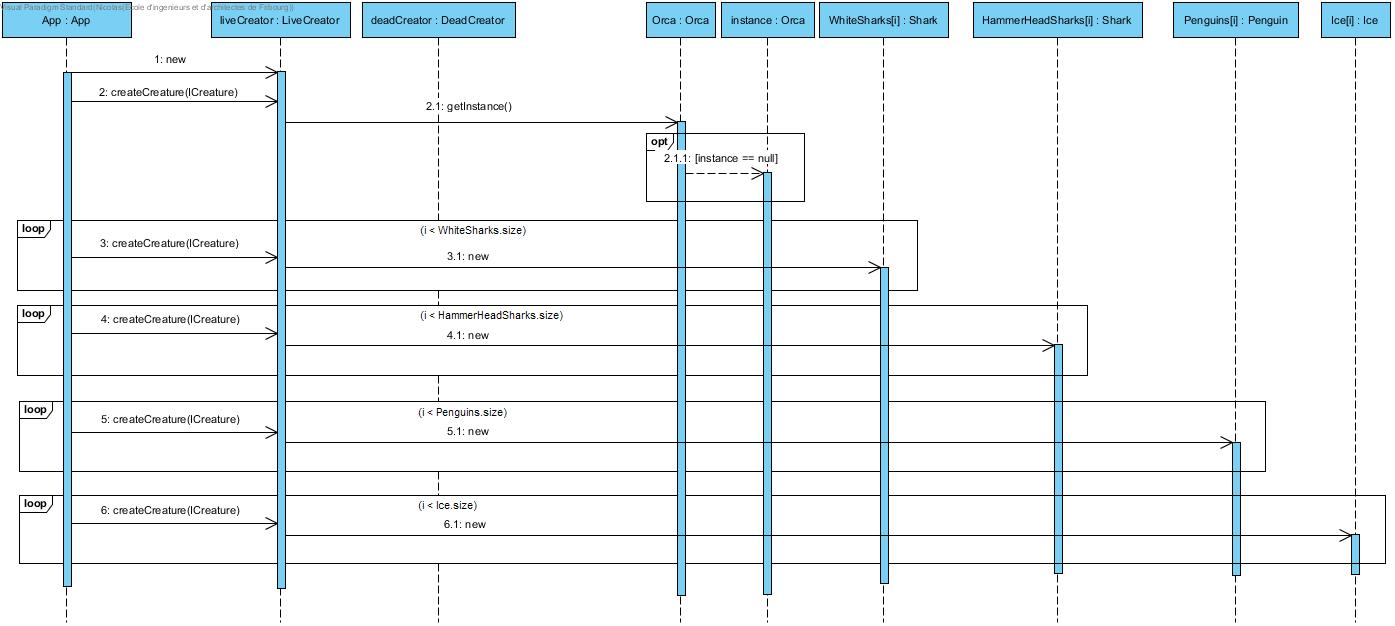
\includegraphics[scale=0.45]{Sequence_r2.jpg}
\end{landscape}



\section{Pattern command}

Nous avons appliqué le pattern command au déplacement que doivent faire les éléments du jeu (move). Pour cela nous l'avons implémenté comme sur le diagramme de classe ci-dessous. \newline

	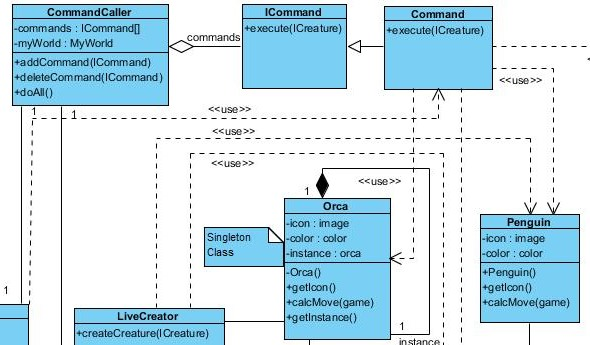
\includegraphics[scale=1]{command.jpg}

\end{document}